\subsection{Heurística Constructiva Golosa}
\subsubsection{Diseño}
\label{sec:greedy-design}
Utilizamos un enfoque \textbf{goloso} a la hora de diseñar este algoritmo, que comienza con una lista ordenada vacía $C$ de camiones (y por ende rutas) fabricando una solución vértice por vértice, es decir, constructivamente. El algoritmo toma como datos de entrada la lista de vértices $V$ que representan los \textit{clientes} que deben ser visitados por los camiones. Su funcionamiento está dividido en cuatro etapas definidas a continuación:

\begin{description}
\item[Paso 1.] Ordenar $V$ por la demanda de cada vértice
\item[Paso 2.] Elegir los vértices de mayor demanda compatibles con el stock disponible de mi último camión en $C$. De no existir ningún vértice con estas características, se despacha el camión al depósito, se invoca uno nuevo con stock lleno y se eligen los vértices más demandantes.
\item[Paso 3.] De la selección previa, se ordenan los vértices por cercanía al \textbf{depósito}
\item[Paso 4.] De estos últimos se escogen $K$ vértices y entre ellos se obtiene el nodo más cercano al camión en cuestión. Este será el siguiente vértice a ser visitado por un camión
\end{description}

\subsubsection{Pseudo-código}
El diseño de este algoritmo fue concebido con el objetivo de minimizar las distancias recorridas por los camiones al intentar vaciarlos lo más rápidamente debido a la temprana atención de los vértices más demandantes. Además de buscar una distancia mínima, con este criterio y bajo ciertas circunstancias también es posible observar una utilización de camiones cercana a la óptima. Pondremos a prueba estos casos más adelante. A continuación, exhibimos el pseudo-código del algoritmo:

\begin{algorithm}[H]
\caption{\Comment $\mathcal{O}(????)$}
\begin{algorithmic}[1]
\Function{resolverCVRP}{Punto $deposito$, Conjunto de puntos $puntos$, Entero $capacidad$}
	\State \textbf{Buckets} $buckets \gets $\textbf{BucketSortPorDemanda}$(puntos)$ \Comment $\mathcal{O}(n + D)$
	\State \textbf{OrdenarCadaBucketPorCercaníaA}$(puntos, deposito)$ \Comment $\mathcal{O}(n*log(n))$
	\Statex
	\State \textbf{Entero} $vertices\_cubiertos \gets 0$
	\State \textbf{Lista de Camiones} $camiones \gets \varnothing$
	\State Insertar en $camiones$ un camión con capacidad $capacidad$ que empieza en $deposito$
	\Statex
	\While{$vertices\_cubiertos < |puntos|$}
		\State \textbf{Bucket} $bucket\_mas\_apto \gets$ \par
        \Statex[3] \textbf{EncontrarBucketMasApto}$(buckets, camiones, deposito, capacidad)$
		\State \textbf{Punto} $siguiente \gets$ \textbf{ExtraerVerticeMasApto}$(bucket\_mas\_apto, camiones)$
		\State Tomar el último camión agregado a $camiones$ y visitar el vértice $siguiente$
		\Statex
		\State $vertices\_cubiertos \gets vertices\_cubiertos + 1$
	\EndWhile

	\State \Return $camiones$
\EndFunction
\end{algorithmic}
\end{algorithm}

\vspace{10 pt}
\fbox{\parbox{0.9\textwidth}{
	Es necesario aclarar que el tipo de datos \textbf{Camión} lleva la cuenta de su stock disponible en forma de \textbf{Entero positivo} y los vértices que visita en un conjunto ordenado de \textbf{Lista de Puntos}. Además, llamamos un \textbf{Bucket} a una \textbf{Lista de Puntos} que comparten la misma demanda. Análogamente, llamamos \textbf{Buckets} a una \textbf{Lista de Buckets}, es decir, Buckets es un alias para una lista de lista de puntos. Hacemos este renombre para resaltar la diferencia entre una lista de puntos con la misma demanda (un bucket) y una lista de puntos cualquiera. El tipo de datos \textbf{Buckets} es obtenido a partir de la invocación de un \textbf{Bucket Sort} sobre una lista de puntos utilizando la demanda de cada vértice como valor comparativo.

	\vskip 8pt

	Como último, el valor $D$ mencionado en la complejidad temporal del \textbf{BucketSort} es la máxima demanda de un punto en la lista $puntos$.
}}
\vspace{10 pt}

\vskip 8pt
Esta función representa la globalidad de la heurística. Comienza realizando un \textit{bucket sort} sobre la demanda de los puntos recibidos por parámetro y luego ordena cada bucket por cercanía al depósito con la función \textbf{OrdenarCadaBucketPorCercaníaA} en la línea 3. La intención de esta heurística es alejarse lo menos posible del depósito, priorizando los vértices más demandantes. Luego, se crea el primer camión y se lo agrega a la respectiva lista. Este camión – como todos – comenzará en el depósito. Luego, el bucle \textit{while} que le sigue intentará encontrar un vértice de demanda máxima que pueda ser satisfecho por el camión. De no encontrarse ninguno, devolverá el camión al depósito e invocará uno nuevo con stock máximo. Esta lógica es delegada en la función \textbf{ExtraerVérticeMásApto}, que devuelve el nodo más demandante posible, invocando o no un nuevo camión si es necesario. Luego, el vértice en cuestión es visitado por el camión y la cantidad de vértices cubiertos es incrementada en uno. El algoritmo se ejecutará $n$ veces, es decir, una vez por cada vértice pues cada iteración visita siempre uno.

\vskip 8pt

\begin{algorithm}[H]
\caption{\Comment $\mathcal{O}(n * log(n))$}
\begin{algorithmic}[1]
\Function{OrdenarCadaBucketPorCercaníaA}{Buckets $buckets$, Punto $punto$}
	\For{\textbf{Bucket} $bucket$ en $buckets$} \Comment $\mathcal{O}(D)$
		\State Ordenar los puntos de $bucket$ por distancia a $punto$ \Comment $\mathcal{O}(|bucket| * log(|bucket|))$
	\EndFor
	\Statex
	\State \Return $buckets$
\EndFunction
\end{algorithmic}
\end{algorithm}

Este algoritmo toma \textbf{Buckets} como parámetro de entrada y, para cada uno de ellos, ordena sus puntos por la distancia al vértice $punto$ adjuntado como dato de entrada. En el contexto general, esta función es utilizada para ordenar todos los vértices de todos los \textit{buckets} por cercanía al depósito del grafo. La complejidad de la estructura de iteración es $\mathcal{O}(D)$ porque dentro de $buckets$ hay $D$ listas de puntos, siendo $D$ la demanda más grande en la lista de puntos del grafo. Luego, la complejidad del sorting de cada bucket depende de la cantidad de elementos dentro de cada uno, es decir: $\mathcal{O}(|bucket| * log(|bucket|))$. Pero es fácil concluir que la complejidad total de esta función es $\mathcal{O}(n * log(n))$ porque a fin de cuentas se están ordenando $n$ vértices en total.

\begin{algorithm}[H]
\caption{\Comment $\mathcal{O}(D)$}
\begin{algorithmic}[1]
\Function{EncontrarBucketMásApto}{Buckets $buckets$, Lista de camiones $camiones$}
	\State \textbf{Entero} $stock\_restante \gets$ stock restante del último camión en $camiones$
	\Statex
	\State \textbf{Entero} $i \gets $\textbf{min}$(stock\_restante, |buckets| - 1)$
	\While{$i \geq 0 \land buckets[i] = \varnothing$}
		\State $i \gets i - 1$
	\EndWhile
	\Statex
	\If{$i < 0$}
		\State Enviar el último camión en $camiones$ al depósito
		\State Creo un nuevo camión en $camiones$
		\Statex
		\State $i \gets |buckets| - 1$
		\While{$buckets[i] = \varnothing$}
			\State $i \gets i - 1$
		\EndWhile
	\EndIf
	\Statex
	\State \Return $buckets[i]$
\EndFunction
\end{algorithmic}
\end{algorithm}

\vspace{10 pt}
\fbox{\parbox{0.9\textwidth}{
	Aclaración: todos los camiones creados inician su ruta en el depósito y con stock lleno. La dimensión de este stock es definida globalmente y es equivalente entre todos los camiones.
}}
\vspace{10 pt}

\vskip 8pt

Esta función se encarga de encontrar el bucket de mayor demanda (pues todos los vértices dentro de este bucket la comparten) tal que pueda ser satisfecha por un camión ya existente o si debe crearse uno nuevo. Su complejidad es $\mathcal{O}(D)$ porque en el peor de los casos, el último camión de la lista no tiene stock suficiente para ningún vértice en el grafo que no haya sido visitado. El primer bucle de la línea 4 comenzará explorando los \textit{buckets} desde el índice $stock\_restante$ hasta llegar a $0$, donde deberá detenerse y concluirá que no hay ningún vértice que cumpla que $demanda(v) \leq stock\_restante$ con $v$ algún vértice en los \textit{buckets} $[0, stock\_restante]$. Luego, se deberá crear un nuevo camión con stock máximo y se volverá a indagar la lista de \textit{buckets}. Sabemos que no hay vértices con demanda en los rangos $[0, stock\_restante]$ pues ya las iteramos en el bucle de la línea 4, pero sabemos que sí quedan vértices sin visitar en el grafo pues sino la función nunca se hubiese ejecutado. Ahora, como por enunciado sabemos que no existe un vértice con una demanda mayor al stock máximo de un camión, sabemos que hay un nodo sin visitar en el rango de índices $[stock\_restante + 1, D]$. En el peor de los casos, el vértice que buscamos está en el índice $stock\_restante + 1$, habiéndose concretado $D$ iteraciones. Finalmente, se retorna el \textit{bucket} en cuestión.

\begin{algorithm}[H]
\caption{\Comment $\mathcal{O}(K*log(K))$}
\begin{algorithmic}[1]
\Function{ExtraerVérticeMásApto}{Bucket $bucket$, Lista de camiones $camiones$, Entero $K$}
	\State \textbf{Punto} $actual \gets$ el último punto visitado por el último camión en $camiones$
	\State Ordenar los últimos $K$ puntos de $bucket$ de más lejano a más cercano a $actual$ \Comment $\mathcal{O}(K*log(K))$
	\Statex
	\State \textbf{Punto} $siguiente \gets$ último elemento de $bucket$ \Comment $\mathcal{O}(1)$
	\State $bucket \gets bucket - \{siguiente\}$ \Comment $\mathcal{O}(1)$
	\Statex
	\State \Return $siguiente$
\EndFunction
\end{algorithmic}
\end{algorithm}

El algoritmo superior recibe un \textit{bucket}, una lista de camiones y un entero $K$. El pedazo de código comienza obteniendo el último vértice visitado por el camión cuya ruta está siendo construída. En base a la posición de este nodo, se ordenan los últimos $K$ vértices de la lista $bucket$ por distancia Euclidiana de más lejano a más cercano. Aquí debemos explicar dos cosas:
\begin{enumerate}[a)]
\item ¿Por qué se ordenan los últimos $K$ vértices de la lista y su completitud? La respuesta a esta pregunta es sencilla: es otra de nuestras \textbf{heurísticas}. No creemos conveniente ordenar todo el \textit{bucket} por cada vértice, por lo tanto lo hacemos con los últimos $K$ ejemplares.
\item ¿Y por qué estos últimos $K$ vértices se ordenan de más lejano a más cercano? Porque sabemos que una vez sea elegido el nodo a visitar, este será removido. Como estamos trabajando sobre un vector, la complejidad de su remoción depende de cuántos elementos le siguen. Como es el último elemento, la complejidad de su remoción es constante.
\end{enumerate}

\subsubsection{Conclusiones}
Podemos entender que como $K$ es un dato heurístico constante, en general pequeño y además menor o igual a $n$ (pues al revés no tendría sentido), su efecto en la complejidad es absorbido por el crecimiento asintótico de $n$, por lo tanto la complejidad queda inafectada por $K$.

\begin{align}
resolverCVRP  &= \mathcal{O}(n+D + n*log(n) + n*D*K*log(K)) \\
              &= \mathcal{O}(n+D + n*log(n) + n*D) \\
              &= \mathcal{O}(n*log(n) + n*D) \\
              &= \mathcal{O}\Big( n*(log(n) + D)\Big) \\
\end{align}

Por otro lado, podemos acotar la complejidad espacial del algoritmo por $\bigO(n)$ porque siempre se trabaja con el conjunto de $n$ vértices y no más.
\subsubsection{Análisis de desempeño}
En esta sección analizaremos las destrezas y debilidades del algoritmo en discusión, que posee al menos dos falencias importantes que pueden producir soluciones de deslucida calidad. A continuación las repasamos:

\subsubsubsection{El algoritmo de \textit{sweeping} no prevee el agotamiento de stock}
A medida que un cluster se va construyendo, la capacidad del camión que atenderá los clientes de este conjunto se va agotando, es decir, la sumatoria de las demandas de todos los clientes en el cluster se va aproximando al valor de la capacidad máxima de los camiones. En estos casos, sería ideal emprender la vuelta hacia el depósito con stock suficiente para satisfacer vértices en el camino. Una manera de entender este concepto es visualizar cada ruta como un pétalo, donde la punta del antófilo indica el comienzo del emprendimiento al depósito. De esta manera, se minimiza la distancia recorrida al volver al punto de inicio pero \textbf{satisfaciendo vértices en el proceso}. Desgraciadamente, el algoritmo es inconsciente de esta situación y, en el peor de los casos, puede agotar su stock muy lejos del depósito solamente por seguir a rajatabla la heurística de viajar al nodo angularmente más cercano, pagando una distancia muy alta para volver.

\vskip 8pt

Esta falencia puede ser mitigada con metaheurísticas como \textbf{Tabú Search} o \textbf{Annealing} a la hora de seleccionar el siguiente vértice a visitar, teniendo en cuenta el vecindario inmediato y la cantidad de stock sobrante en el camión.

\begin{figure}[H]
	\centering
	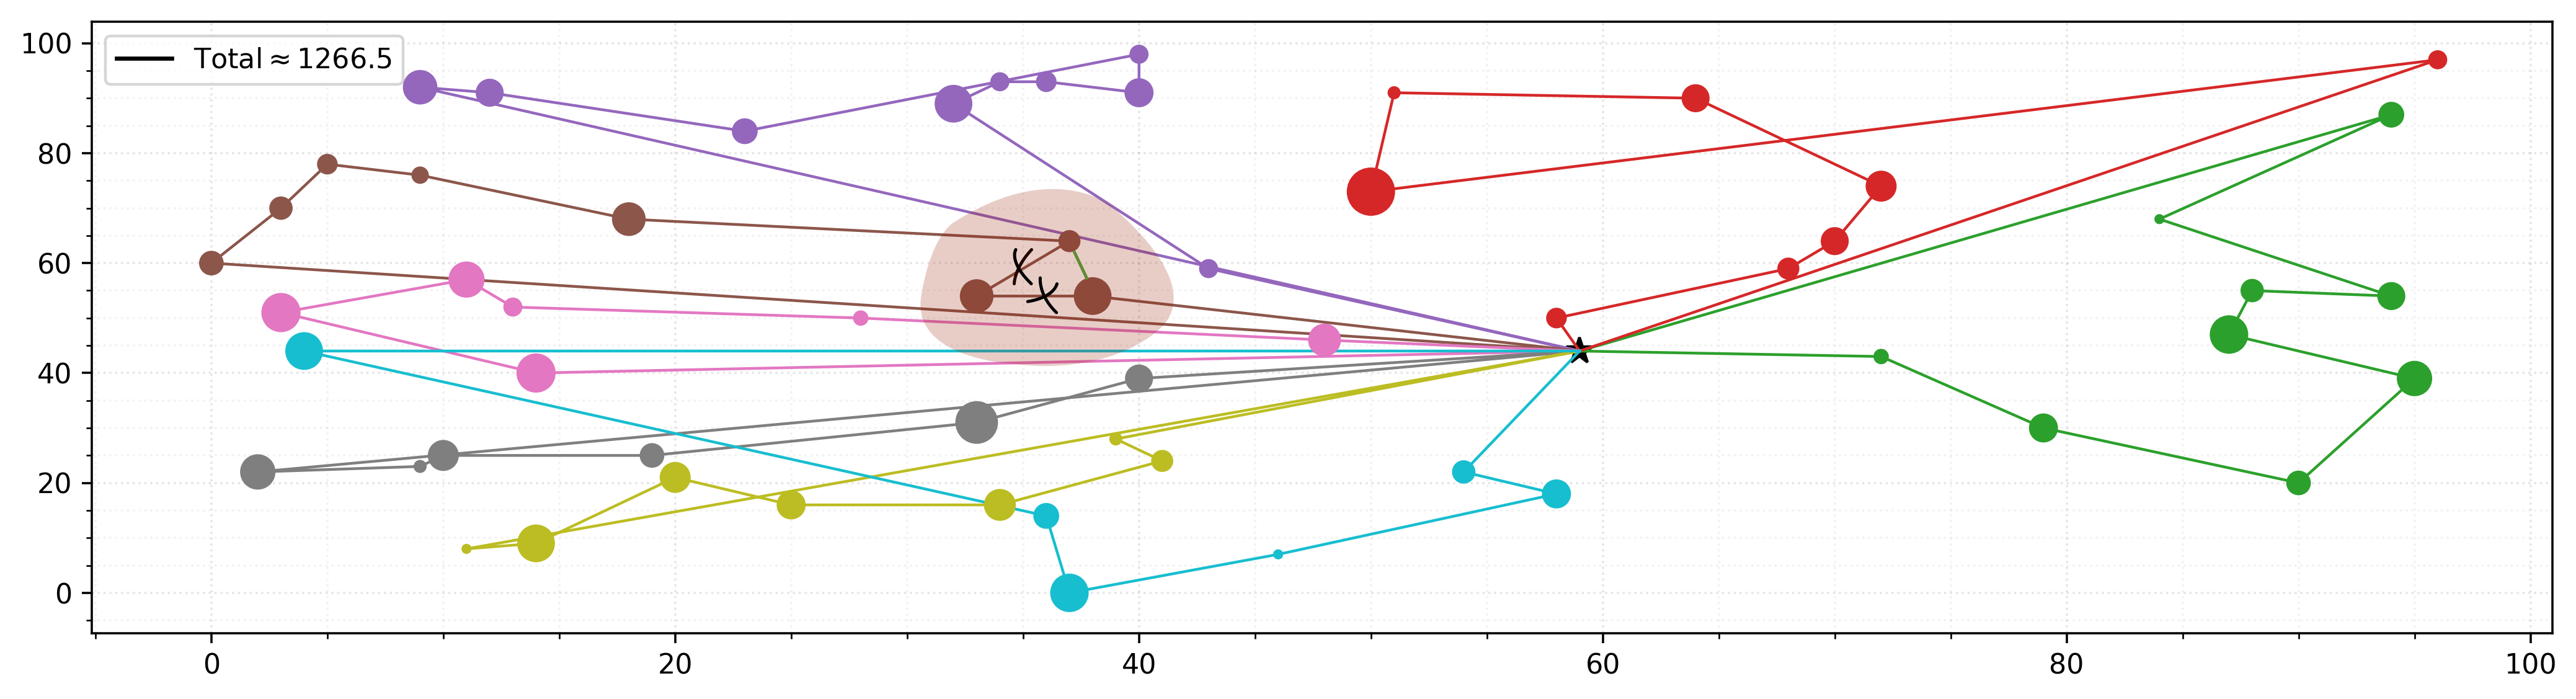
\includegraphics[width=1\textwidth]{sweep/A-n69-k9-emprender-vuelta}
	\caption{\footnotesize Error de optimización en la generación del camino (dataset A-n69-k9)}
	\label{fig:sweep-emprender-vuelta}
\end{figure}

En la figura \ref{fig:sweep-emprender-vuelta} se puede observar que en el camino marrón es posible obtener un mejor recorrido al eliminar los ejes marcados con una cruz y, en cambio, agregando la arista verde como figura en el gráfico. De esta manera quedaría un vértice $v$ sin conectar. Luego, si observamos el eje $e$ formado por el depósito y el nodo más alejado a él en esta ruta, podemos generar una subdivisión de la arista $e$ con el vértice $v$ concluyendo en un camino más óptimo. En resumen: la solución del gráfico \ref{fig:sweep-emprender-vuelta} posee una ruta que realiza un \textit{paso hacia atrás}, alejándose de los nodos que tiene que visitar después y tomando posesión de un cliente que podría haber sido visitado a la hora de \textbf{emprender la vuelta} hacia el depósito. Este ejemplo es uno de los muchos que puede suceder en esta familia de problemas.

\subsubsubsection{La heurística de \textit{TSP} puede ser muy golosa con las distancias}
Debido a que el orden de los clientes en los clusters es resuelto a través de la heurística \textit{Nearest Neighbours} que consiste en visitar el nodo inmediatamente más cercano sobre el cual se está parado, se puede perder el panorama general y cometer decisiones costosas para la calidad de la solución final. El ejemplo más recurrente se ve en la presencia de rutas con bucles o \textit{firuletes}, pues se produce una ``ida y vuelta'' innecesaria con total de visitar el nodo más cercano posible. Esto podría ser evitado utilizado alguna metaheurística como Annealing o Tabú Search para decidir a qué vértice saltar o utilizar una técnica como Lambda Exchange para optimizar e intentar eliminar estas manifestaciones del problema descripto. Analizaremos este fenómeno gráficamente:

% \newpage
\parindent0em
\begin{multicols}{2}[\columnsep2em]
		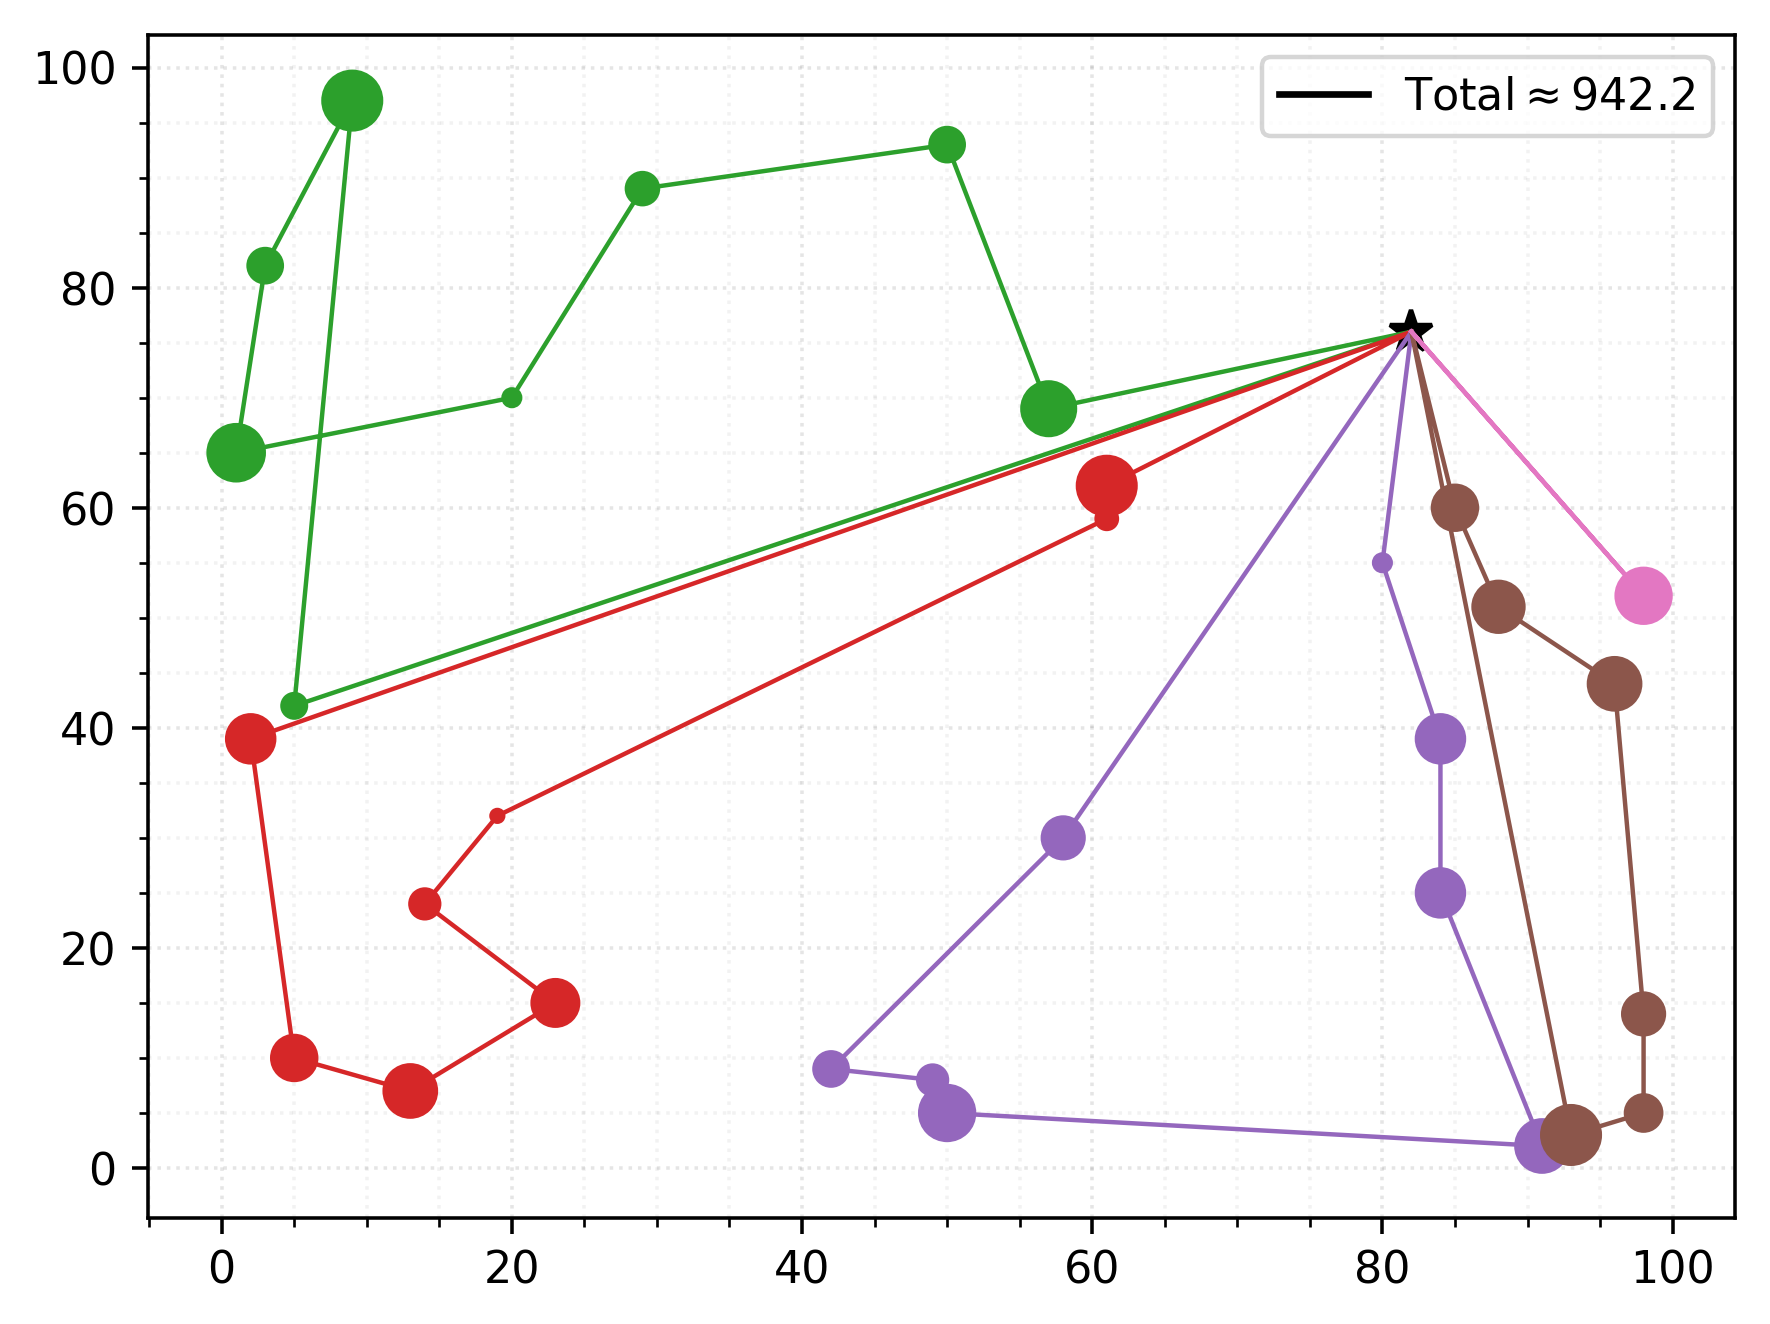
\includegraphics[width=0.48\textwidth]{sweep/sweep-A-n32-k5}
\columnbreak
	\begin{figure}[H]
		\caption{Circuito no óptimo en camino verde} \label{fig:sweep-A-n32-k5}
		\vskip 4pt
		En este ejemplo se puede ver claramente la aparición de un circuito en la ruta verde. Como ya fue explicado, este se debe a que el algoritmo de resolución del TSP busca los nodos inmediatamente más cercanos sin considerar otras alternativas (a priori más ineficientes) pero que a la larga resultan más óptimas. Al seguir a rajatabla la heurística de \textit{Nearest Neighbours}, se comete un error de \textit{tunnel view} y se ignoran alternativas más eficientes a la larga.
	\end{figure}
\end{multicols}

\subsubsubsection{Clusterización con sweeping adaptativo vs sin sweeping adaptativo}
En la figura \ref{fig:sweep-with-adaptative} se puede observar una clusterización correcta de los vértices. Los nodos recorridos por el camión verde son cercanos entre sí y lo mismo sucede con los del camión rojo. En cambio, en la figura \ref{fig:sweep-without-adaptative}, se puede observar cómo los clusters se interponen entre sí debido a que se comenzó a barrer angularmente sobre ángulo $0$, interrumpiendo a la mitad la concepción de un cluster óptimo.
\begin{figure}[H]
	\centering
	\begin{minipage}{0.48\textwidth}
		\centering
		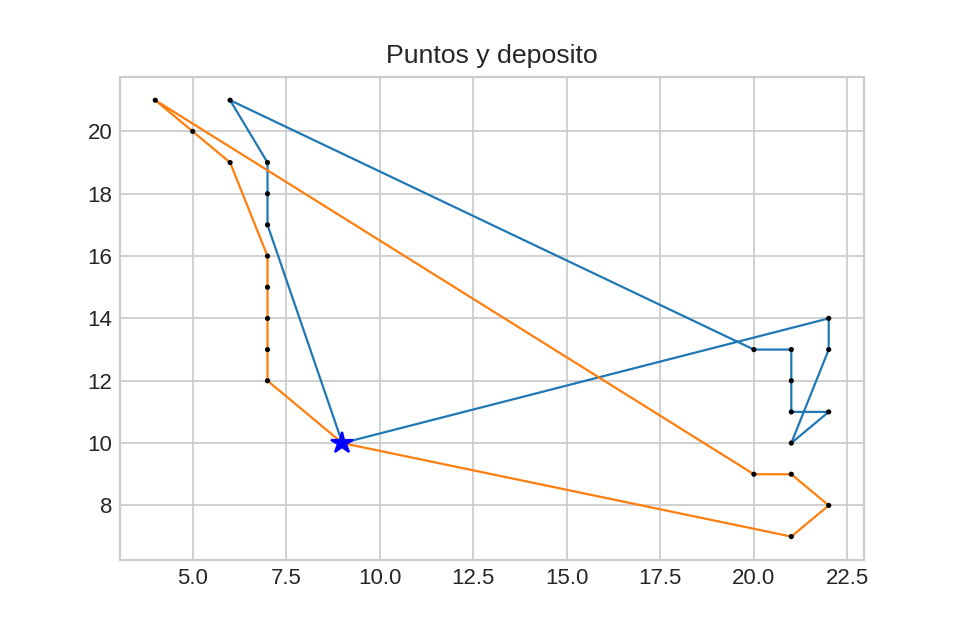
\includegraphics[width=1\textwidth]{sweep/sweep-without-adaptative}
		\caption{\footnotesize Sweeping no adaptativo}
		\label{fig:sweep-without-adaptative}
	\end{minipage}%
	\hspace{0.03\textwidth}
	\begin{minipage}{0.48\textwidth}
		\centering
		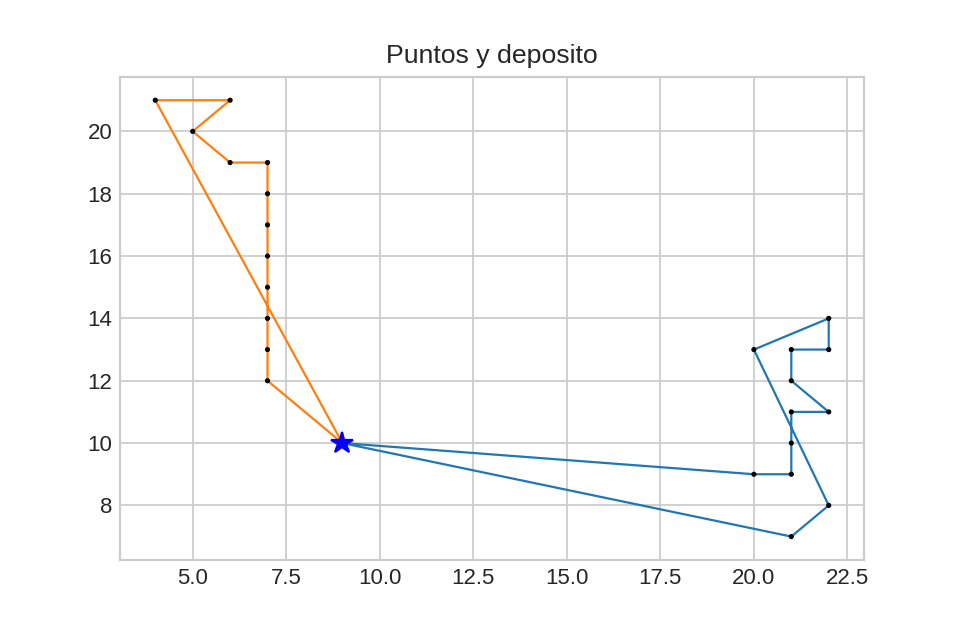
\includegraphics[width=1\textwidth]{sweep/sweep-with-adaptative}
		\caption{\footnotesize Sweeping adaptativo}
		\label{fig:sweep-with-adaptative}
	\end{minipage}%
\end{figure}

\subsubsubsection{El barrido angular puede clusterizar vértices muy lejanos entre sí}
Dada la clusterizaciónn de vértices $V=\{v_{1}, \dots, v_{n}\}$ realizada por la heurística de Sweeping donde, si bien está asegurado que la distancia angular desde el depósito entre todo $v_{i}$ y $v_{i+1}$ con $1 \leq i < n$ es mínima en todo el grafo, no está asegurado que la distancia euclidiana entre $v_{i}$ y $v_{i+1}$ sea mínima también. De hecho, la distancia entre $v_{i}$ y $v_{i+1}$ puede ser arbitraria. Sin embargo, al clusterizar ambos vértices juntos, estamos firmando un contrato donde un solo camión deberá proveer a ambos y esto puede ser extremadamente costoso por más que los recorridos sean realizados a fin de cuentas con una heurística de TSP. Veamos un ejemplo:

\begin{figure}[H]
	\centering
	\begin{minipage}{0.48\textwidth}
		\centering
		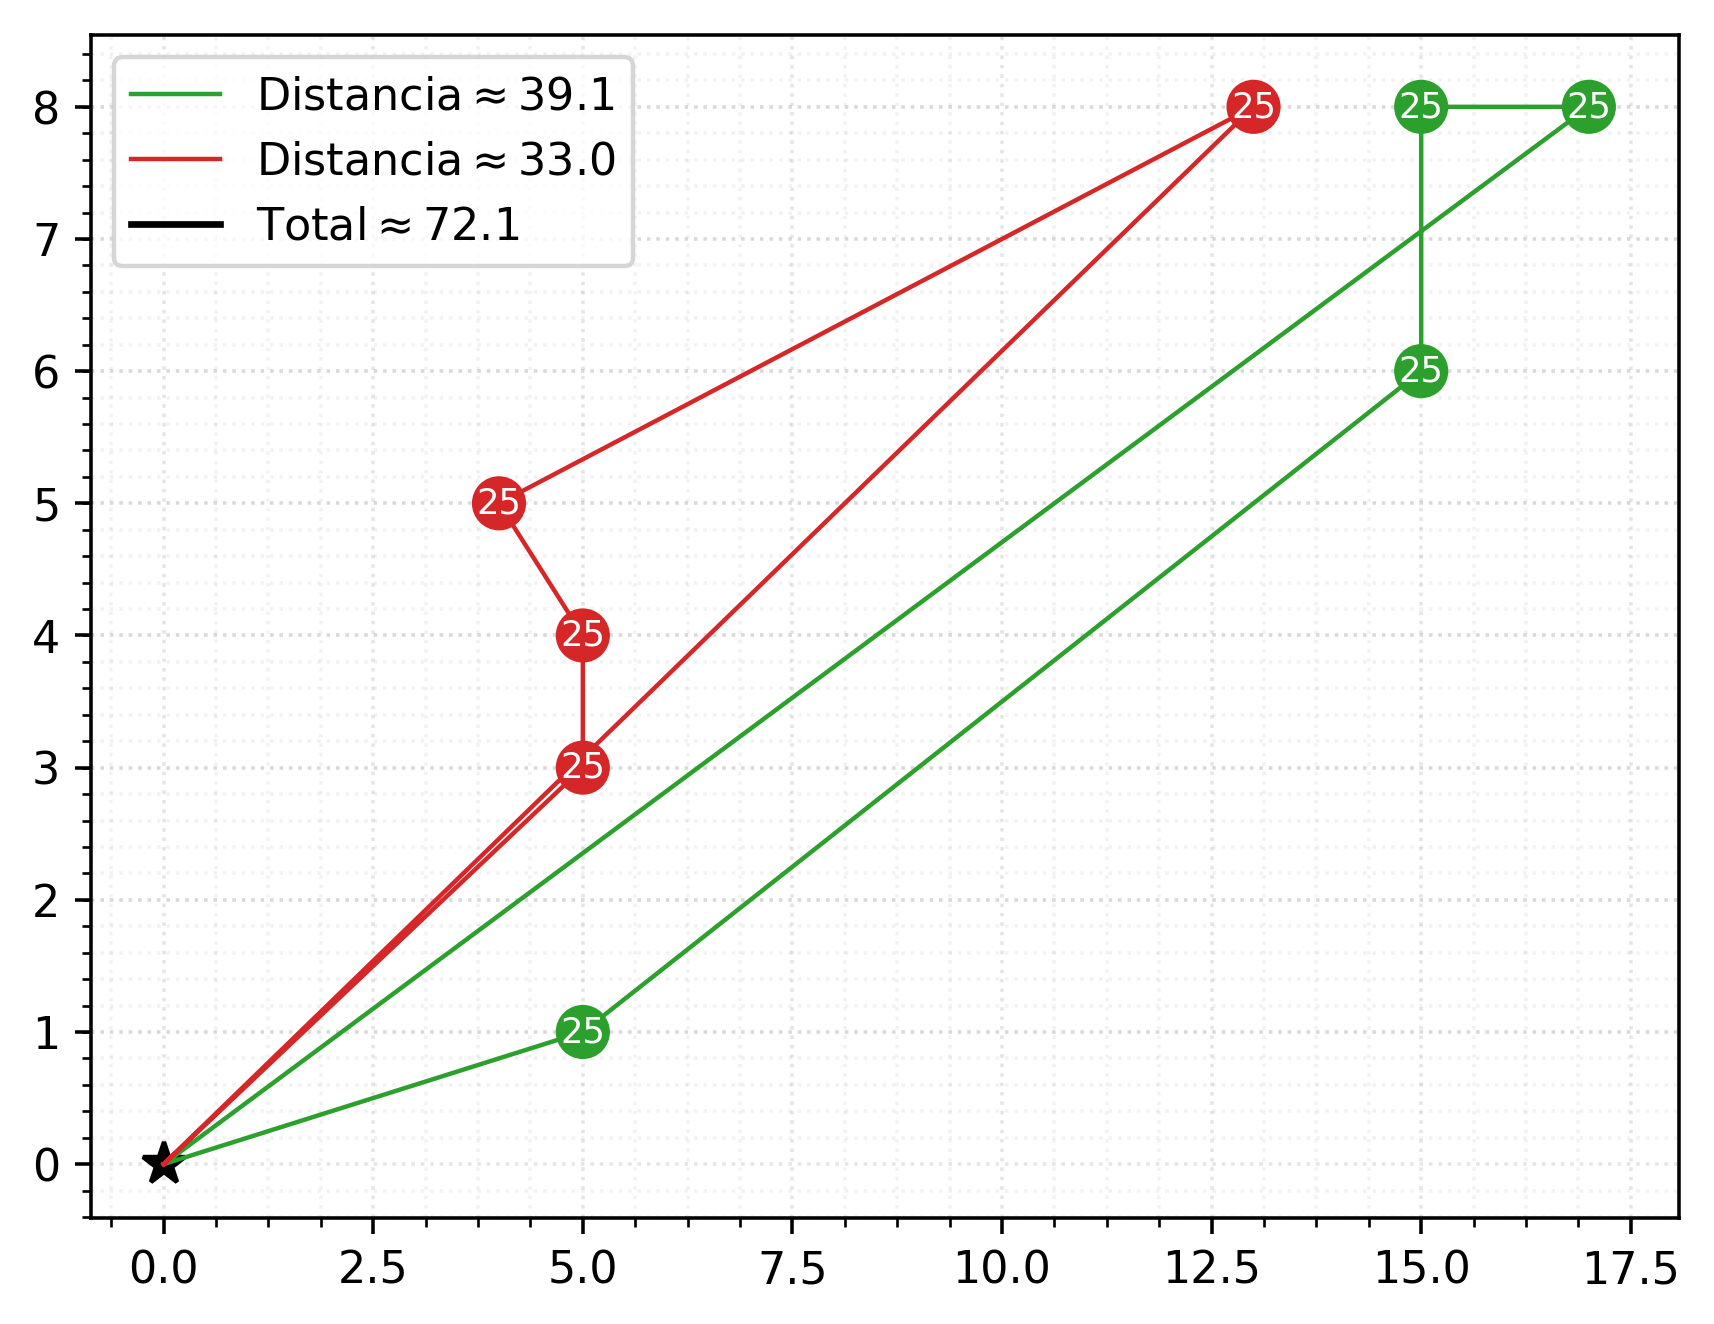
\includegraphics[width=1\textwidth]{sweep/sw-custom-n9-sweep-close-angular-far-euclidean}
		\caption{\footnotesize Sweeping + Nearest Neighbours. Capacidad 100.}
		\label{fig:sw-custom-n9-sweep-close-angular-far-euclidean}
	\end{minipage}%
	\hspace{0.03\textwidth}
	\begin{minipage}{0.48\textwidth}
		\centering
		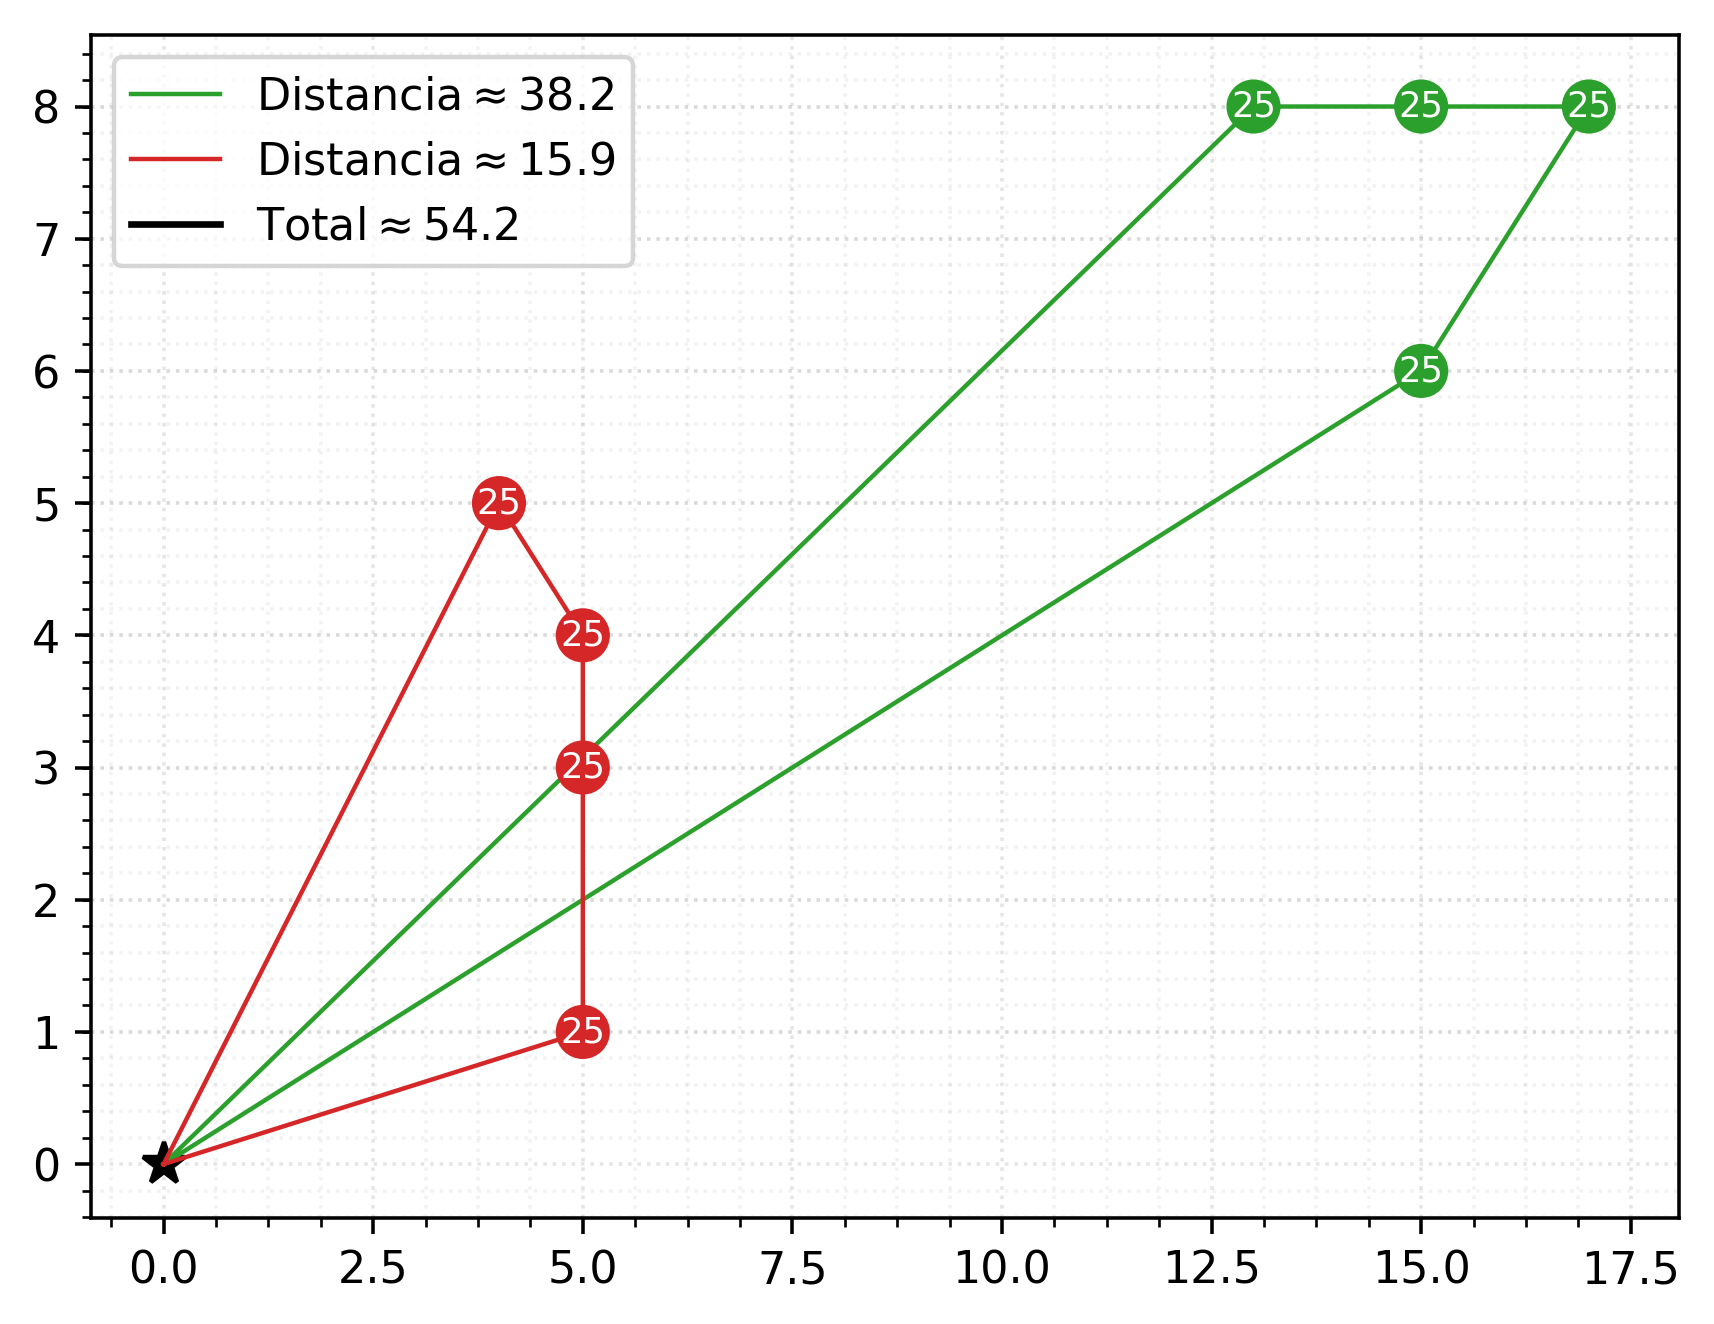
\includegraphics[width=1\textwidth]{sweep/km-custom-n9-sweep-close-angular-far-euclidean}
		\caption{\footnotesize K-Means + Nearest Neighbours. Capacidad 100.}
		\label{fig:km-custom-n9-sweep-close-angular-far-euclidean}
	\end{minipage}%
\end{figure}

En este caso se puede observar claramente lo mencionado. La solución con \textit{sweeping} encuentra primero el vértice $(5, 1)$ e inmediatamente después el $(15, 6)$, seguido del $(17, 8)$ y cierra el cluster con $(15, 8)$. Luego ya se disponen de 4 vértices cuya demanda suma $100$, la capacidad máxima de un camión. Esto forma un cluster de cuatro vértices donde uno de ellos está muy lejos de los otros tres pues estos cuatro son consecutivos angularmente pero \textbf{no} euclideanamente. Lo mismo sucede con los otros cuatro vértices sobrantes del grafo. En consecuencia, se consume mucha distancia yendo y viniendo de aquellos vértices lejanos del resto. En cambio, en la figura \ref{fig:km-custom-n9-sweep-close-angular-far-euclidean} se puede observar una distribución más natural de las rutas y, en consecuencia, un decremento en la distancia total recorrida por ellas. Esto se debe a que se utilizó la heurística de clusterización \textbf{K-Means} que resulta \textbf{más apropiada para la instancia del problema} pues – como será explicado más adelante – construye los clusters a partir de la distancia euclideana entre sus vértices y no sus distancias angulares al depósito.

